%% Document-wide settings.
\documentclass[letterpaper]{article}
\title{Latex article template}
\author{Thomas HOULLIER} 

\usepackage[colorlinks=true, allcolors=blue,
            hyperfootnotes=false,
            pdfauthor={Thomas HOULLIER},
            pdftitle={Latex article template},
	    pdfkeywords={<keywords>}]
            {hyperref} % Links for ref/cite.

%% Loading packages
\usepackage{amsmath} % For cases in equations.
\usepackage{amsfonts} % For maths sets.
\usepackage{physics} % For \abs{} and \norm{}.
\usepackage{svg} %svg graphics
\usepackage{siunitx} % units formatting

\usepackage[backend=biber,style=numeric,citestyle=numeric-comp,maxcitenames=99,dateabbrev=false]{biblatex}
\addbibresource{biblio.bib}
\usepackage{setspace} % Bibliography spacings
\DeclareSourcemap{
  \maps[datatype=bibtex]{
    \map[overwrite]{
      \step[fieldsource=doi, final]
      \step[fieldset=url, null]
      \step[fieldset=eprint, null] }}}
\setcounter{biburllcpenalty}{7000} % break long url in bibliography
\setcounter{biburlucpenalty}{8000}
\renewcommand*{\bibfont}{\footnotesize} % bibliography font size
% Format of biblatex urldate in the bibliography.
\DeclareFieldFormat{urldate}{%
  Visited on \thefield{urlday}\addspace%
  \mkbibmonth{\thefield{urlmonth}}\addspace%
  \thefield{urlyear}\isdot}
\usepackage[ruled,vlined]{algorithm2e} % Algorithms.
\usepackage{algorithmic}
\usepackage{mathtools} % Ceiling function.
\usepackage{outlines} % Nest lists.
\usepackage{interval} % Writing intervals.
\usepackage[font={footnotesize,sf}]{caption} %Caption for figures in minipages.
\usepackage{floatrow}
% Figure captions always below. Figures always centered.
\floatsetup[figure]{capposition=bottom,objectset=centering}
\usepackage{wrapfig} %Wrapping figure with text.
\usepackage{stmaryrd} % Double brackets for integers interval.
\usepackage{doi} % Hyperlink DOI
\usepackage{etoolbox} %Ragged right bibliography.
\usepackage{color, colortbl} % Coloring rows in tables.
\usepackage{subcaption} % Subfigures.
\usepackage{pdfpages} % Include PDF pages.
\usepackage{epigraph} % Quotations at beginning of chapters.
\setlength\epigraphwidth{.8\textwidth}
\usepackage[acronym,nonumberlist,nogroupskip,nopostdot]{glossaries} % Glossary for acronyms.
\renewcommand*{\glstextformat}[1]{\textcolor{black}{#1}} % No color on links for abbrev.

\usepackage[capitalise,nameinlink]{cleveref} % Include eg. "Fig." in front of figures.
\crefname{algorithm}{Alg.}{Algs.}
\crefname{table}{Tab.}{Tabs.}
\crefname{equation}{Eq}{Eqs.}
% Equation cross-references.
%\creflabelformat{equation}{#2#1#3}
\crefformat{equation}{(#2Eq.\thinspace#1#3)}

% No parentheses in equation labels.
%\newtagform{noparen}{}{}
%\usetagform{noparen}

\DeclarePairedDelimiter{\ceil}{\lceil}{\rceil} % Ceiling function.
\DeclarePairedDelimiter{\floor}{\lfloor}{\rfloor} % Floor function.

\DeclareMathOperator*{\argmin}{argmin}

\setcounter{tocdepth}{3} % Table of content depth
\setcounter{secnumdepth}{3} % Section numbering depth

% Non-breaking around footnotes.
\makeatletter
\let\Footnote\footnote
\def\pst@@killglue{\unskip\ifdim\lastskip>\z@\expandafter\pst@@killglue\fi}
\def\footnote{\pst@@killglue\Footnote}
\makeatother

% More space below equations
\appto\normalsize{\belowdisplayshortskip=\belowdisplayskip}

% Rewrite month codes in bibliography
\DeclareSourcemap{
  \maps[datatype=bibtex]{
    \map[overwrite]{
      \step[fieldsource=month, match=\regexp{\A(j|J)an(uary)?\Z}, replace=1]
      \step[fieldsource=month, match=\regexp{\A(f|F)eb(ruary)?\Z}, replace=2]
      \step[fieldsource=month, match=\regexp{\A(m|M)ar(ch)?\Z}, replace=3]
      \step[fieldsource=month, match=\regexp{\A(a|A)pr(il)?\Z}, replace=4]
      \step[fieldsource=month, match=\regexp{\A(m|M)ay\Z}, replace=5]
      \step[fieldsource=month, match=\regexp{\A(j|J)un(e)?\Z}, replace=6]
      \step[fieldsource=month, match=\regexp{\A(j|J)ul(y)?\Z}, replace=7]
      \step[fieldsource=month, match=\regexp{\A(a|A)ug(ust)?\Z}, replace=8]
      \step[fieldsource=month, match=\regexp{\A(s|S)ep(tember)?\Z}, replace=9]
      \step[fieldsource=month, match=\regexp{\A(o|O)ct(ober)?\Z}, replace=10]
      \step[fieldsource=month, match=\regexp{\A(n|N)ov(ember)?\Z}, replace=11]
      \step[fieldsource=month, match=\regexp{\A(d|D)ec(ember)?\Z}, replace=12]}}}

% Footnotes marker color
\renewcommand\thefootnote{\textcolor{blue}{\arabic{footnote}}}

\pdfsuppresswarningpagegroup=1 % Silence warnings about pagegroups for figures.
\pdfminorversion=6 % PDF version 1.6 since we include articles in 1.6.

% Allow an extra pass to fix overfull hboxes by allowing more whitespace.
\emergencystretch=1em

% Page numbering and copyright notice.
\usepackage{fancyhdr}
\usepackage{lastpage}

\fancypagestyle{FirstPage}{
\fancyhf{} % Clear footer.
\rfoot{\thepage \hspace{1pt} of \pageref*{LastPage}}
\renewcommand{\headrulewidth}{0pt} % Remove rule at top of page
\lfoot{\href{https://creativecommons.org/licenses/by/4.0/}
       {\includesvg[inkscapelatex=false,height=14pt]{images/ccby.svg}}}}

\fancypagestyle{plain}{
\fancyhf{} % Clear footer.
\rfoot{\thepage \hspace{1pt} of \pageref*{LastPage}}
\renewcommand{\headrulewidth}{0pt} % Remove rule at top of page
}

% Version history
\usepackage{vhistory}

% Keywords
\providecommand{\keywords}[1]{\textbf{Keywords --} #1}

% Glossary
\makeglossaries
\loadglsentries{glossary/glossary.tex}


% Document
\begin{document}
\frenchspacing
\date{v1.0 -- \today}
\maketitle

\begin{abstract}
We provide a LaTeX article template. It is meant for scientific writing in
article format.
\end{abstract}

\keywords{LaTeX, Documentation, Article, Technical writing.}

\begin{versionhistory}
\vhEntry{1.0}{\today}{TH}{creation}
\end{versionhistory}
\setcounter{table}{0} % Reset the table counter.

\tableofcontents
\printglossary[type=\acronymtype,style=index]
\thispagestyle{FirstPage}
\pagestyle{plain}
\section{Examples}
We provide examples of some of the latex features and packages we use most.
This is both a visual check that our template formats things the way we
want to, and a reference on how to use relevant LaTeX features.

\subsection{Citation}
Citations are made in the following way:
\begin{itemize}
\item Single citation: \cite{Gehrels:2016}.
\item Two citations: \cite{inkscape,gnuplot}.
\item Citations list: \cite{inkscape,gnuplot,thomashoullier/alarm-clock}
\end{itemize}

The bibliography will automatically only include the references which
were cited in the document.

\subsection{Acronyms}
Acronyms are defined in a list at the beginning of the document. Only
actually used acronyms are included. The acronyms are defined in the text
automatically the first time they are used.

For instance:
\begin{itemize}
\item First use: \gls{RBF}.
\item Subsequent uses: \gls{RBF}.
\end{itemize}

\subsection{Equations}
Equations are written in the usual manner (see
\cref{eq:example,eq:example2,eq:example3}).

\begin{equation} \label{eq:example}
\int_{a}^{b} \omega(x) f(x) \approx \sum_{i=1}^n w_i f(x_i)
\end{equation}

\begin{equation} \label{eq:example2}
\begin{cases}
p_{n+1}(x) = (A_n x + B_n) p_n(x) - C_n p_{n-1}(x) \\
p_0(x) = 1 \\
p_1(x) = A_0 x + B_0
\end{cases}
\end{equation}

\begin{equation} \label{eq:example3}
e^{ - at} \cos (\Omega t)u(t) \Leftrightarrow
\frac{{s + a}}{{(s + a)^2  + \Omega ^2 }}
\end{equation}

See the LaTeX equation examples at \cite{equationsheet,SO-latex-equations}.

\subsection{Figures}
Figures have the following appearance (see \cref{fig:svg,fig:sinus,fig:photo}).

\begin{figure}
\includesvg[width=.6\textwidth]{images/inkscape-logo.svg}
\caption{\label{fig:svg} Example vector image in svg format. This is the
Inkscape™ logo. Inkscape is a \gls{svg} editor \cite{inkscape}.}
\end{figure}

\begin{figure}
\includesvg[width=.7\textwidth]{images/gp-sin/sinus.svg}
\caption{\label{fig:sinus} Example plot in svg format. Created using gnuplot
\cite{gnuplot}.}
\end{figure}

\begin{figure}
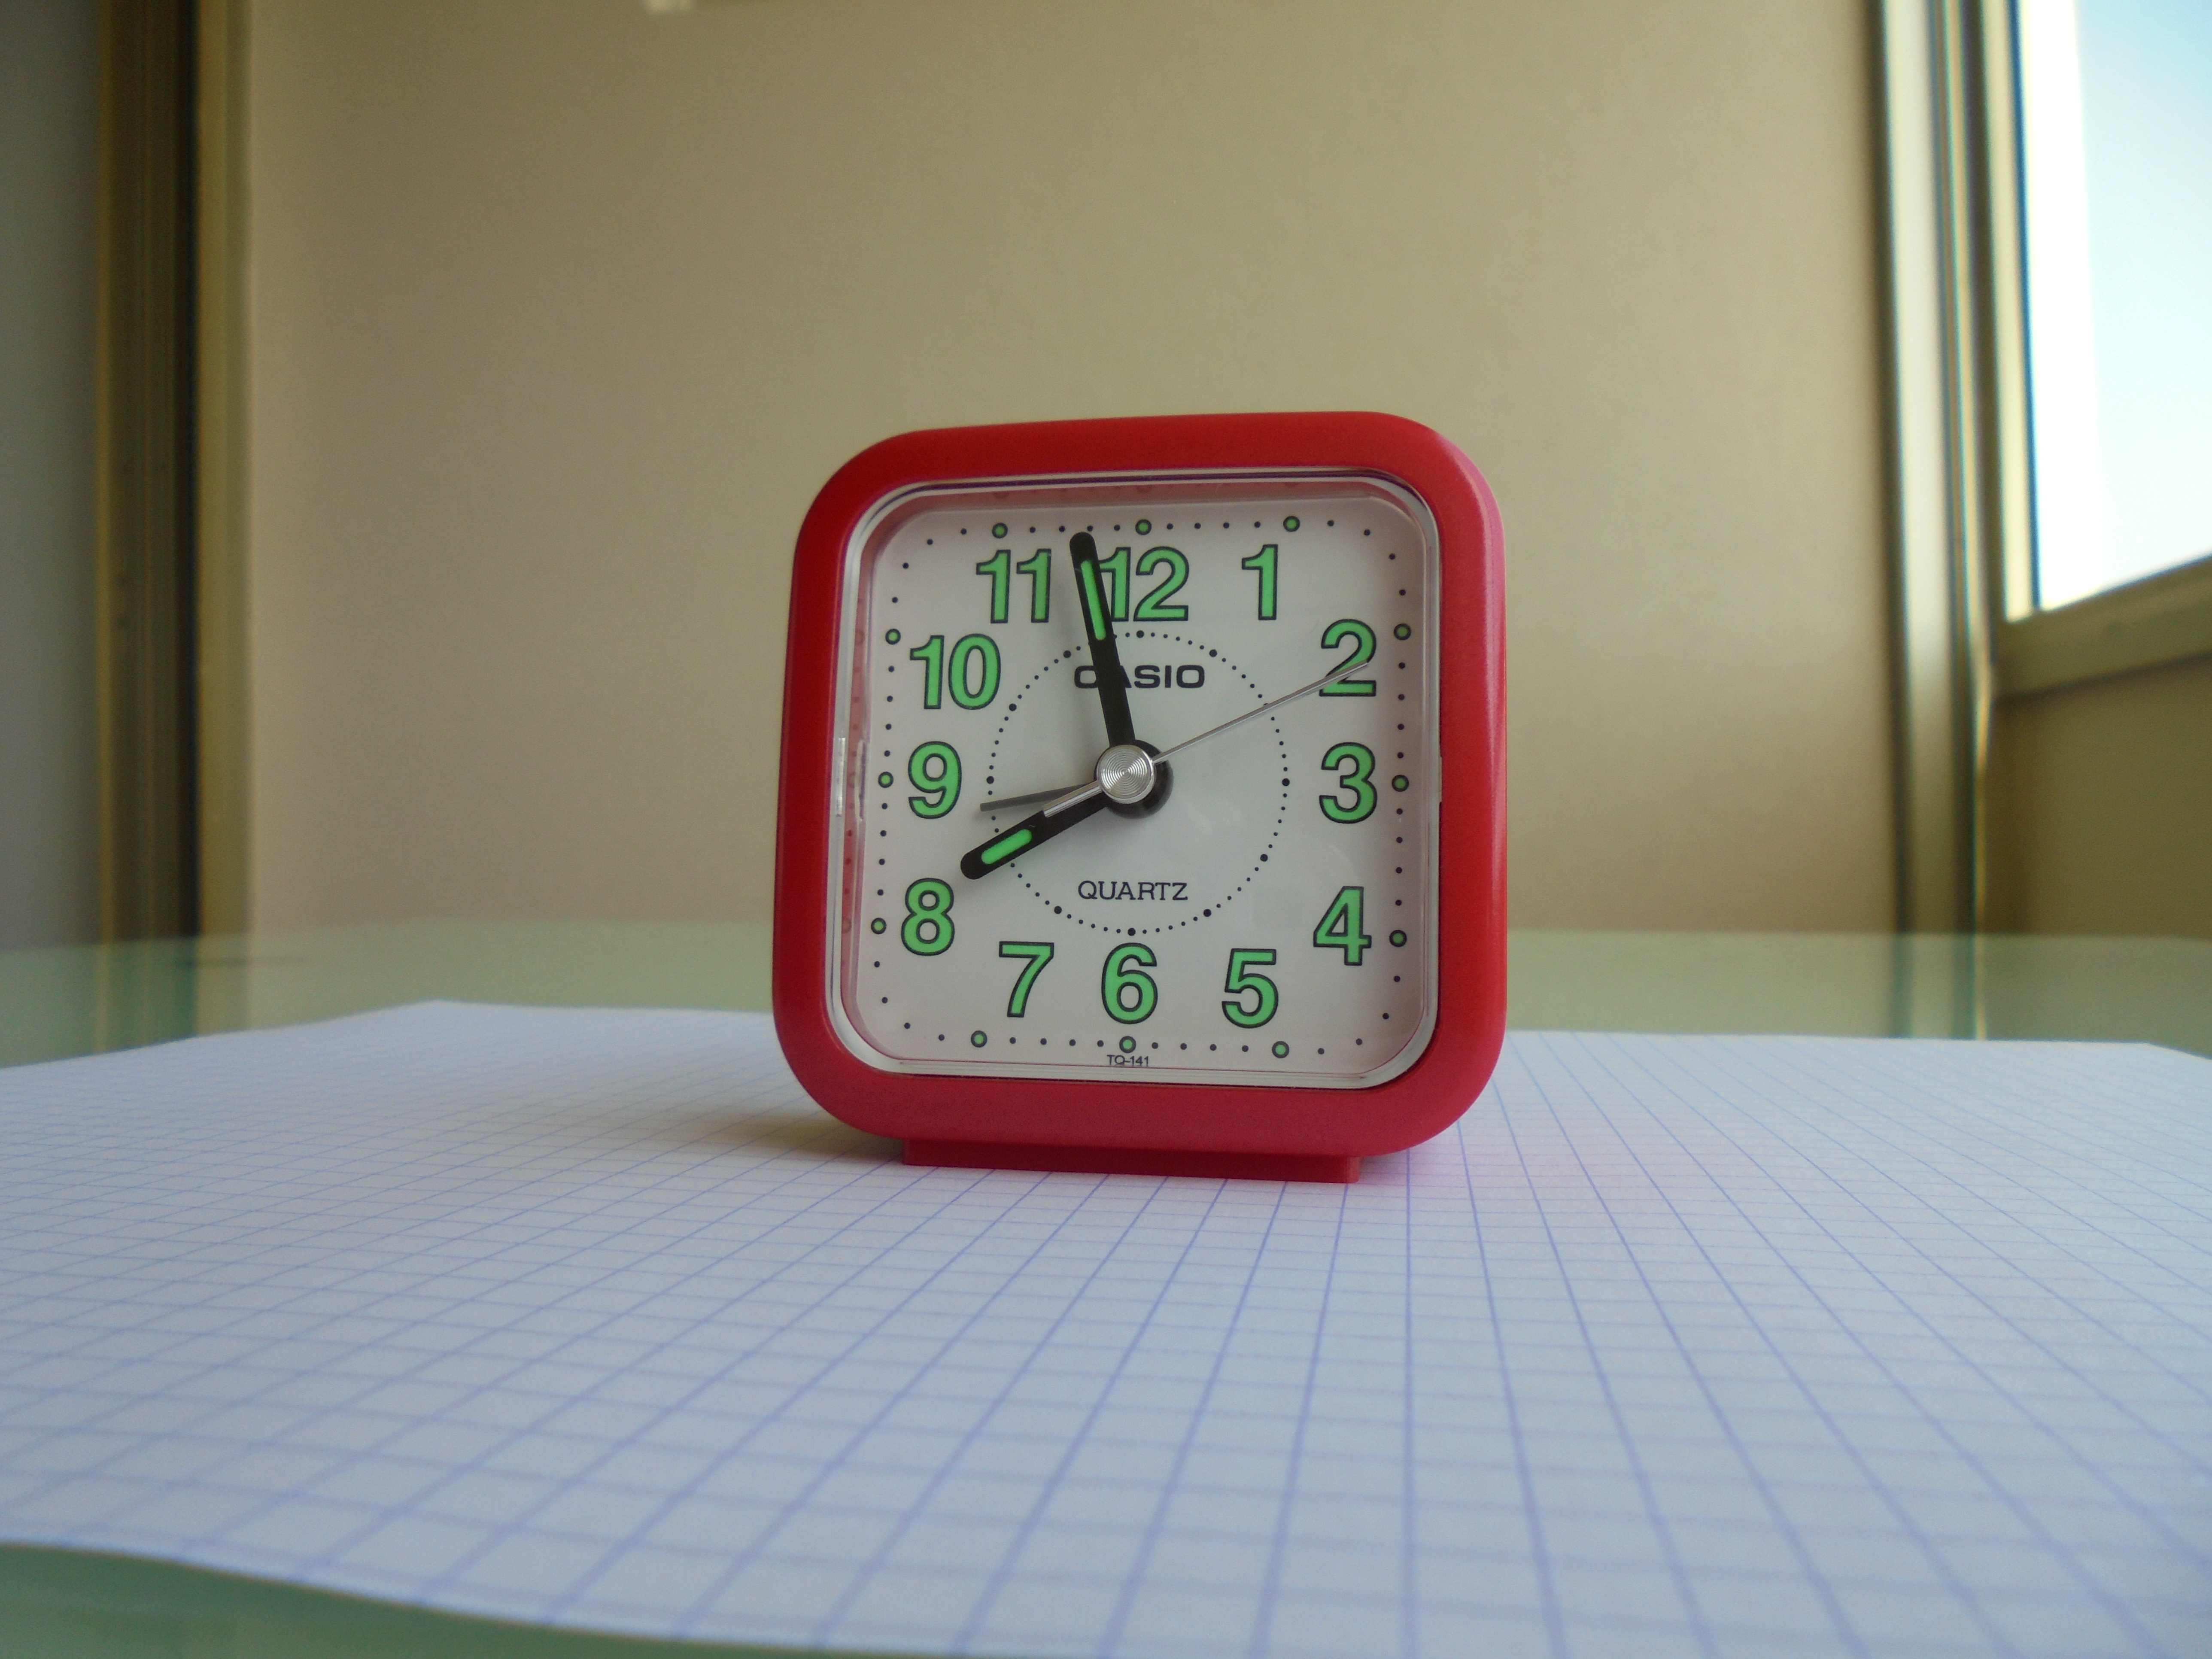
\includegraphics[width=\textwidth]{images/photo-alarm-clock.jpg}
\caption{\label{fig:photo} Example raster image: photography from the
project \cite{thomashoullier/alarm-clock}.}
\end{figure}

My own rules of thumb regarding the format of images are:
\begin{itemize}
\item \textbf{Vector images}, such as \gls{svg}: I use \gls{svg} as much
as possible. I find this important with respect to the feeling of quality
a document inspires. I make an exception for images with a number of elements
that would be excessive for document rendering.
\begin{itemize}
\item Diagrams: can be edited with Inkscape \cite{inkscape}.
\item Plots: can be generated by gnuplot \cite{gnuplot}.
\item Logos: Most logos have a vector version.
\end{itemize}
\item \textbf{Raster images}
\begin{itemize}
\item Photographs: Raster representations are well suited to photographs.
      Most photographs should be compressed, depending on what the author
      wants to show, so as not to add unnecessary weight to the output document.
      The tool jpegoptim \cite{tjko/jpegoptim} is well suited for this purpose.
      I find both \gls{jpg} and WEBP formats to give good results.
\item Screenshots: Screenshots generally contain large areas filled with a
      single color. \gls{png} and WEBP are recommended here.
\end{itemize}
\end{itemize}

\subsection{Tables}
Tables may be created in the following way (see
\cref{tab:example1,tab:example2,tab:example3}).

\begin{table} \caption{\label{tab:example1} Example table.}
\begin{tabular}{l | c c c} \hline
1 & a & b & c \\ \hline
2 & d & e & f \\ \hline
3 & g & h & i \\
\hline \end{tabular}
\end{table}

\begin{table} \caption{\label{tab:example2} Example table: second.}
\begin{tabular}{l | c c c} \hline
4 & j & k & l \\ \hline
5 & m & n & o \\ \hline
6 & p & q & r \\
\hline \end{tabular}
\end{table}

\begin{table} \caption{\label{tab:example3} Example table: third.}
\begin{tabular}{l | c c c} \hline
7 & s & t & u \\ \hline
8 & v & w & x \\ \hline
9 & y & z & $\chi$ \\
\hline \end{tabular}
\end{table}

\subsection{Algorithms}
Algorithms may be typeset as follows \cref{alg:euclid-gcd}.

\begin{algorithm}
\caption{\label{alg:euclid-gcd} Euclid's algorithm for \gls{GCD}
\cite{enwiki:euclid-algorithm}.}
\SetKwInOut{Input}{Input}\SetKwInOut{Output}{Output}

\Input{$(A, B) \in \mathbb{N}$}
\KwResult{$\text{gcd}(A, B)$}
\BlankLine
$X \gets A$\;
$Y \gets B$\;
\While{$X \neq Y$}{
  \eIf{$X > Y$}
    {$X \gets X - Y$}
    {$Y \gets Y - X$}}
\KwRet{$X$}
\end{algorithm}

\subsection{Inline code and Blocks of code}
Inline code: \lstinline[style=mystyle,language=sh]{cat /etc/group}. Blocks of code are
\cref{lst:python,lst:octave,lst:common-lisp}.

\begin{lstlisting}[language=Python,
                   caption={Python code sample \cite{numpy-hfft}.},
                   label={lst:python}]
>>> signal = np.array([1, 2, 3, 4, 3, 2])
>>> np.fft.fft(signal)
array([15.+0.j,  -4.+0.j,   0.+0.j,  -1.-0.j,   0.+0.j,  -4.+0.j]) # may vary

>>> np.fft.hfft(signal[:4]) # Input first half of signal
array([15.,  -4.,   0.,  -1.,   0.,  -4.])

>>> np.fft.hfft(signal, 6)  # Input entire signal and truncate
array([15.,  -4.,   0.,  -1.,   0.,  -4.])
\end{lstlisting}

\begin{lstlisting}[language=Octave,
                   caption={Octave code sample \cite{octave-example}.},
                   label={lst:octave}]
m = rows (A); n = columns (A);
[U, S, V] = svd (A);
## determine the regularization factor alpha
## alpha =
## transform to orthogonal basis
b = U'*b;
## Use the standard formula, replacing A with S.
## S is diagonal, so the following will be very fast and accurate.
x = (S'*S + alpha^2 * eye (n)) \ (S' * b);
## transform to solution basis
x = V*x;
\end{lstlisting}

\begin{lstlisting}[language=Lisp,
                   caption={Common Lisp code sample
                            \cite{common-lisp-example}.},
                   label={lst:common-lisp}]
(defun entropy (string &aux (length (length string)))
  (declare (type string string))
  (let ((table (make-hash-table)))
    (loop for char across string
          do (incf (gethash char table 0)))
    (- (loop for freq being each hash-value in table
             for freq/length = (/ freq length)
             sum (* freq/length (log freq/length 2))))))
\end{lstlisting}

\subsection{Footnotes}
Footnotes may be included in this fashion\footnote{Hello}.

\subsection{Epigraphs}
\epigraph{Respondeo dicendum quod necesse est dicere spiritum sanctum a filio
esse. Si enim non esset ab eo, nullo modo posset ab eo personaliter distingui.}
{Sanctus Thomas Aquinas -- Summa Theologiae I, q.36, a.2}

Epigraphs can be included. They are meant for the beginning of sections.

\subsection{Icons}
The fontawesome package \cite{fontawesome-latex} may be used for small icons
in-line with the text \faSmileO~\faMedkit~\faBicycle.

\subsection{Cross-references}
We list cases of cross-referencing to check how they look.

\begin{itemize}
\item Equations
\begin{itemize}
  \item Single: \cref{eq:example}.
  \item Two: \cref{eq:example,eq:example2}.
  \item List: \cref{eq:example,eq:example2,eq:example3}.
\end{itemize}
\item Figures
\begin{itemize}
  \item Single: \cref{fig:svg}.
  \item Two: \cref{fig:svg,fig:sinus}.
  \item List: \cref{fig:svg,fig:sinus,fig:photo}
\end{itemize}
\item Tables
\begin{itemize}
  \item Single: \cref{tab:example1}.
  \item Two: \cref{tab:example1,tab:example2}.
  \item List: \cref{tab:example1,tab:example2,tab:example3}.
\end{itemize}
\item Algorithms
\begin{itemize}
  \item Single: \cref{alg:euclid-gcd}
  \item Two:
  \item List:
\end{itemize}
\item Listings
\begin{itemize}
  \item Single: \cref{lst:python}
  \item Two: \cref{lst:octave,lst:python}
  \item List: \cref{lst:octave,lst:python,lst:common-lisp}
\end{itemize} \end{itemize}


\section{Usage}
We detail how a PDF of the present template may be generated.


\appendix
\cleardoublepage

%% \include{appendices}

\apptocmd{\thebibliography}{\raggedright}{}{}
\begingroup
\setstretch{0.6}
\setlength\bibitemsep{0pt}
\printbibliography
\endgroup
\end{document}
